
\chapter{Reference Model Construction}
%%%%%%%%%%

This chapter conceptions the process reference model and is central part of this thesis. In order to discuss particular processes, the framework itself needs to be discussed. What follows is the discussion of processes, which puts special emphasis on design decisions, \viz \textit{how} to model certain aspects with constructs of the language icebricks. 

	%%%%%%%%%%
	deloitte W14: managing change dispute:::: innovation und so... wichtig für begründung des frameworks
	\section{Process Framework}
	
	\citeauthor{Meise2001} defines a framework as \enquote{an ordering relevant elements and relationships on a high level of abstraction. [...] Purpose is to give an overview about an original and to support structuring of elements and relationships on lower detail levels} \citep[\p{62}]{Meise2001}. Drawing further on his work, which especially targets framework design in process-oriented organizations, the proposed procedure for construction is adopted (\Fig \ref{fig:meise}). Differences to his approach arise, as the reference model should display as as-is state of the domain and does not follow goals of reorganization set by a specific company. Therefore, the \textit{organization} represents a fictive BPO provider in CRM in the following, which captures generic aspects of the domain. The construction is split into two components. The structural part first encompasses strategic and fundamental reflections, while the graphical component transfers these into a visual form that supports communication.

	\begin{figure}[caption={procedure for framework construction}, label={fig:meise}]
		{	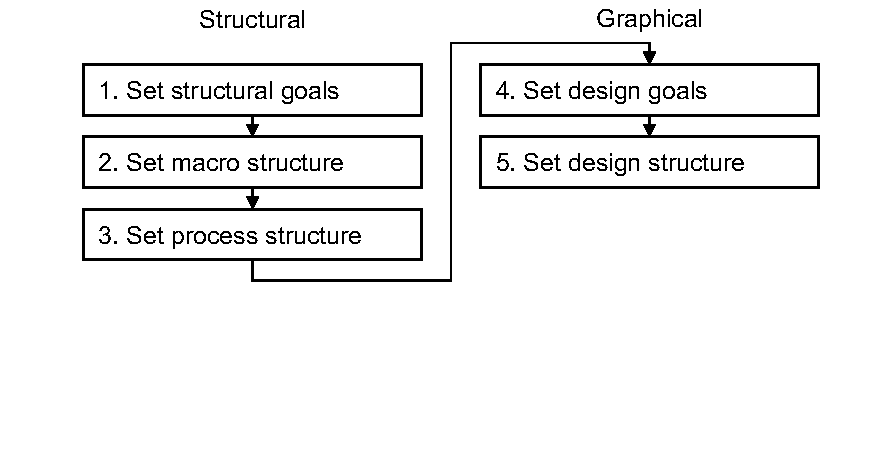
\includegraphics[width=.8\textwidth]{figures/framework-meise.pdf}}
		\hspace{6.2cm}	SOURCE:  adapted from \citep[\p{122}]{Meise2001}
	\end{figure} 
	
	\subsection{Set structural goals}
	
	Modeling is no end in itself and different purposes require different models. Theoretically speaking, purpose of this research is to create an artifact that generates utility and tackles a problem in the real-world.  Previously identified problems (\ref{sec:proide}) lead to objectives (\ref{sec:solobj}) which are to be faced with the process reference model in general and its framework in particular. The existence of general (organizational) and stakeholder-related objectives requires the framework to bring together both ends, as it is the basis of the model. 
	
	\begin{table}[caption={Solution Objectives}, label={tab:solobj}]
		\centering
		\begin{tabular}{l p{13.3cm}}

			\textbf{No. }&\textbf{ Solution Objective}
			 \\ \hline
			\textbf{1 }                        & Construction of a generic reference model that covers distinguishing processes for BPO-providers in CRM on concept level.                                                    \\ \hline
			\textbf{2}                         & The reference model can be applied for use at Arvato CRM.                                                                                                                    \\ \hline
			\textbf{3 }                        & The construction,process is well-documented, makes use of empirical research by induction, which is enriched by deduction from \acrshort{BPO} and \acrshort{CRM} theory. \\ \hline
			\textbf{4}                         & A syntactic and semantic formalized process modeling language is used, that is transferable to other languages.                                                              \\ \hline
			\textbf{5}                         & The model can be used as a statement of competence for sales activities towards clients.                                                                                     \\ \hline
			\textbf{6}                         & The model holds a process representation, which supports a common understanding across client businesses.                                                                    \\ \hline
			\textbf{7}                         & The model is able to represent an omni-channel environment.                                                                                                                 
		\end{tabular}
	\end{table}

	
	
	\subsection{Set macro structure}
	
	A framework, as a strategic tool, incorporates concepts of strategy. One can name two perspectives, namely a market- or resource-based view of strategy, which are directed externally or internally, respectively. They are not independently of each other, but their interplay is seen as an important factor in strategic decision making. \cite{becker2004handelsinformationssysteme} note, that standardization in keeping with reference model application has contra-productive effects on strategic competitive advantages. This argument is true, when the reference model is used as a application model. The application of the reference should incorporate strategic characteristics of the company, which implies that this reference model framework can only capture a strategic orientation as perceived useful by the author. 
	
	The market-based view follow the structure-conduct-performance paradigm, that explains success of a company through external factors in the industry. \cite{porter1980} formulated the so called five-forces model, which describes bargaining power of suppliers (1), threat of substitutes (2), bargaining power of buyers (3), threats of new entrants (4) and industry rivalry (5) as determinants of competition. Applying these two the BPO domain, a trivial substitute for outsourced services is the return of services inside the parent organization. Further, the substitution of customer services through automation may render outsourcing obsolete. The bargaining power of suppliers and buyers can be loosely mapped to clients and customers. While clients as suppliers clearly influence the provider directly, customers show less of this influence on the outsourcing provider. As the provider takes an intermediate position between client and customer (\cf \Fig \ref{fig:bpochain}), their acting is always in connection with the client. However, an assessment of outsourced service quality puts pressure originating from the customer on the provider, which in turn will also be judged by the client. The entry of new players on the market (4) can be tackled by barriers, that go back to competitive advantages of differentiation or cost-leadership. While the latter is especially causing fierce competition in low-wage regions that realize offshore-outsourcing, outsourcing players in CRM that feature more profound services, lean towards a differentiation strategy. This can also be stated for Arvato. Lastly, industry rivalry among players in the BPO CRM market is also influenced by the aforementioned generic strategies, to position established companies. A framework adopts market-based aspects through accounting for markets or segments therein. These are accompanied by business units or processes that relate to this external environment. 
	
	The resource-based view of strategy analyzes internal strengths and weaknesses. Resources are bundled to form capabilities and should be rare, inimitable, create value and be non-substitutable. Due to asymmetries of resources, competitive advantages are enabled. The identification of capabilities of CRM BPO providers (\cf \ref{sec:bpocrmis}: operational and business development capabilities) can only be done on a generic level for the reference model. Application necessitates specifying the framework to conform to company-specific capabilities. The operational capability should reflect the operational process component in CRM (\cf \ref{crmprocessfr}), and service delivery from the outsourcing side (\cf \ref{app:provproc}). Business development, \ie understanding and addressing client needs, misses a pendant in an isolated CRM view, but can be put in relation to delivery management in the outsourcing model. 
	
	Putting both views together emphasizes the client and customer market environment and two capabilities, that relate to these markets. Towards the client side, providers are criticized by clients for being too reactive instead of proactive (49\%), delivering poor service quality (48\%) and lack of innovation (37\%) \citep{deloitte2014outsourcing}. While the first point of criticism addresses the client relationship, the other two are directed towards the service itself. Looking at the constituents of \acrshort{CRM}, the people, process, technology split draws a line to the resource-based view, as these three resources need to be developed and captured to enable superior service provision for clients. Apart from the  \acrshort{CRM} view, these three also have their own meaning in \acrshort{BPO}. The importance of processes in  \acrshort{BPO} is obvious. The people component can be interpreted here as the provision of manpower and their training for services; (information) technology as an enabler of outsourcing (\cf \ref{sec:bpo}) . 
	
		
	\subsection{Set process structure}
	\label{sec:procstr}
	Given that the model shows processes, the structural split of people, processes and technology is hardly meaningful, as two aspects of  \acrshort{CRM} or \acrshort{BPO} would be left out. Drawing from the BPO chain and the identified stakeholders enables another categorization that leaves room for design choices, while capturing generic aspects of business processes within \acrshort{BPO}. As \acrshort{BPO} is the framing construct and  \acrshort{CRM} one use of it, this order is to be prioritized. The following briefly describes business processes, that are detailed in the remainder of this chapter.
	
	
	\begin{figure}[caption={BPO chain provider scope with stakeholders}, label={fig:bpochainscope}]
		{	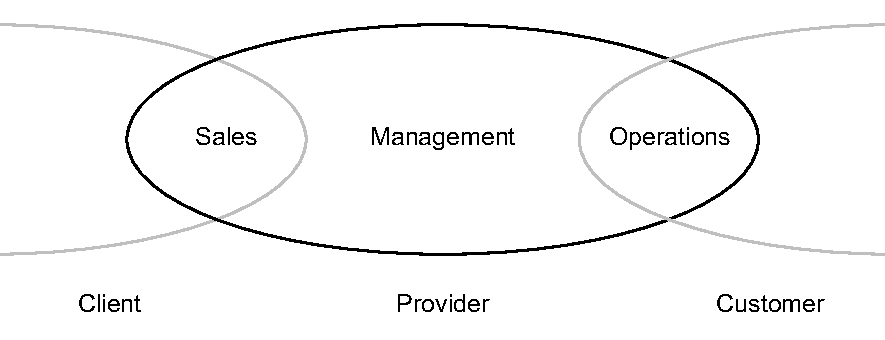
\includegraphics[width=.8\textwidth]{figures/chain2.pdf}}
	\end{figure} 
	
	\subsubsection{Sales-related}
	Sales-related business processes cover processes that have touchpoints with the client. These take place along a lifecycle, which starts with initial contact between provider and client, and hopefully advances through creation of an outsourcing contract. For this agreement, the \acrshort{BPO} provider places its products (\ie, service blueprints) in the clients requirements profile, so create solutions for identified problems. Also, the implementation and setup of the outsourced business must take place. After everything is set up, the client relationship is maintained under the umbrella of account management. 
	
	\subsubsection{Management-related}
	The management-related business processes bring together resources in the provider organization, so that the operations and business development capability are realized. Regarding the latter, it is important to have a products in place, which can be implemented as service solutions for clients.  \citep{schewe2007} names this delivery management, but explicitly refers to its similarities with product development. In addition to the development, the management of existing products inside a product portfolio becomes important. The operations capability can be addressed by processes, that enable economies of scale. Benefits through economies of scope are a question of offered services and not processes. Economies of scale are realized by the increased output of services across client businesses, which in turn necessitates alignment in these services so that their output can be counted \enquote{together}. This alignment is facilitated through a product-view of services and their underlying portfolio in the organization. In addition, people in the provider organization need to be trained  in order to excel in the role of \acrshort{CSR}. Their career path can be seen from a process perspective, so that a strong relationship is established with their employer. This aspect shall be called People Lifecycle Management\footnote{The term people is preferred over agent or \acrshort{CSR}, because it puts this process strongly in connection \acrshort{CRM}. As the management-related processes are tried to be references for \acrshort{BPO} in general, this is not intended.} Lastly, management of the workforce, especially scheduling, becomes critical in a business like customer service. The assurance of the right capacity at the right time to meet fluctuating demand with little waiting time is expected from the client. Therefore, efficient techniques to manage the complexity of multiple channels, different demand patterns and differently skilled \acrshort{CSR}s are necessary. This is encapsulated in the process of workforce management. 
	
	\subsubsection{Operations-related}
	The last group of business processes target the service delivery in the words of \citeauthor{schewe2007}. The processing of transactions with customers is in focus, which can be on numerous channels. A transaction in this case is a conversation, so that theories of communication \citep{shannon1949} may be used here.  A message is sent from a sender to a receiver through a medium. In case of customer service, both the customer or the \acrshort{CSR} can start a conversation, that has a subject which relates to the client in some way. Reasons for contact may be separated by being related to a previous transaction. This transaction might be a purchase of a client's good or service. The communication channel increasingly varies and is no reasonable split, as in an omni-channel environment a seamless experience across channels is intended. Hence, the processes should be similar on a high level of abstraction. 
	
	Communication can be asynchronous (\eg, e-mail) or synchronous(\eg, voice), which puts emphasis on temporal differences in the conversation. While the employed process definition encompasses the \enquote{time-logical sequence of activities}, the value(\viz time between activities) does not impact the process logic itself, as this is a question of succession. General steps in inquiry handling from a business perspective will be similar independent of the (a)synchronous case. What becomes more important from a business perspective is the question who initiates the customer contact. A communication triggered by the customer (incoming) follows demand patterns that are inferred from historic data, while better planning of \acrshort{CSR} opened contacts (outgoing) is possible, as the temporal decision of contact lies at the business and not the customer. 
	
	Lastly, one has to differentiate in customer contact whether \acrshort{CSR}s are involved in inquiry handling, which obviously has business implications. When customers use self-service to address their needs, software takes the \acrshort{CSR} role, which saves resources. Providers can differentiate themselves through expertise in these systems. Clients save money by less volume that is processed by humans (employees of the outsourcing provider). At first sight, this may cannibalize outsourcing business, but the expertise of installing and running these self-service systems is often not located in clients that outsource \acrshort{CRM}. Consequently, providers can generate new business by accumulating know-how in self-service activities. On the one hand, they design the customer-facing self-service in order to handle the inquiry (which by definition are customer-initiated). On the other hand, the provider manages and maintains the knowledge base, that sits behind these automatons in the back-end. This knowledge management does not only have implications on self-service, but also on other customer contacts, as the \acrshort{CSR}s in the human-to-human communication also query the knowledge base to solve customer problems.  
	
	It is desisted from the explicit modeling of a customer journey, because it encompasses components that cannot be part of a process model for providers. The model in this thesis is centered on the outsourcing provider. Modeling of a customer journey requires a customer-centric model, which then contains steps of the customer journey in a detailed way. Such a model should be a \textit{playground} for identifying space for improvement in dialog with a client regarding its customer journey. In addition, it would benefit from avoiding the standards of process models, as its purpose is seen in the \textit{design} of a journey through \acrshort{CRM} components. Research from the field of marketing can be found \citep{Lemon_2016, Frow_2007}. 
	
	\subsection{Set design goals}
	
	The visual representation of the framework is linked to its cognition among viewers, therefore it needs to support the communication of the reference model's purpose. In contrast to language-processing, the process of perception is foregrounded, as the graphic is processed all at once and not sequentially. The model has to capture the fundamental characteristics of the domain of outsourcing at first glance. The sketched model level when applied (provider and client model) should be visually supported, as the framework of the reference is the blueprint to convey this hierarchy. 
	
	\hfill\begin{minipage}{\dimexpr\textwidth-1.2cm}
		\textbf{Design Goal 1}: The framework has to visualize the business of BPO providers.
	\end{minipage}

From a process perspective, as well as to reduce complexity, it helps to highlight important business processes over supporting or coordinating processes. By doing this, the viewer gets an impression about central parts of the model. 

	\hfill\begin{minipage}{\dimexpr\textwidth-1.2cm}
	\textbf{Design Goal 2}: The framework has distinguish business processes from other process types. 
\end{minipage}

Furthermore, the provisioned services are to be shown. In order to gain an understanding of characteristics in CRM outsourcing, especially in an omni-channel context, the framework has to clearly communicate their orientation towards the customer. As it is the differentiating aspect towards BPO for other processes, this fact could be incorporated in the design.  

	\hfill\begin{minipage}{\dimexpr\textwidth-1.2cm}
	\textbf{Design Goal 3}: The framework has to cover the CRM-orientation in service provision. 
\end{minipage}

A framework's purpose is to manage complexity by displaying relevant elements. In addition, the visual representation should be clear, consistent and structured to enable understanding on its own. 

	\hfill\begin{minipage}{\dimexpr\textwidth-1.2cm}
	\textbf{Design Goal 4}: The framework has to be easily processable by viewers without further explanation. 
\end{minipage}


	visualize the business of BPO providers
	distinguish business processes from other process types
	encapture CRM orientation 
	be easily processable by viewers without further explanation
	
	
	
	\subsection{Set design structure}
	
	The design of the reference model primarily addresses reference model users. However, its design will have large influence on the depiction of an application model. It is noted that the framework is designed independent of a process modeling language. The use of reference design (model) can serve as a basis, it is brings with it benefits that have been previously discussed in context of reference models. The house reference design for example is used in the Retail-H (\ref{mod:retail}). Known patterns influence human perception \citep{kroeber1997} and can transfer associations. In the case of the house reference design, one can link solidity, stability and security \citep[\p{216}]{Meise2001} with it. It is made up on three parts (\viz roof, core, foundation), which can be used to visualize coordination, main and supporting processes, respectively. The foundation represents a basis on which the house is build. Its main part, biggest in size, stands in the center and has the largest impact on the perception of the house's content. The roof brings together underlying elements and has an analogy towards an organizational hierarchy. 
	
	\subsubsection{Framework composition}
	
	Adding the previously discussed process structure, supported by the BPO-chain design, one can convey this representation into the core area. \Fig \ref{fig:frameworkdesign} shows influences for the framework areas. 
	\citeauthor{Meise2001} proposes the use of a value chain representation with a chevron that enables linking of multiple elements, which is called a \acrfull{VACD}. It communicates the input, transformation, output relation of a company, as the area on the left or right hand side of the house can be used to model supply or distribution markets. 
	These two markets are existing in BPO with end-customer interaction (like in \acrshort{CRM}), which nicely brings together house reference design and \acrshort{BPO}-chain. 
	
	\begin{figure}[caption={Framework design influences}, label={fig:frameworkdesign}]
		{	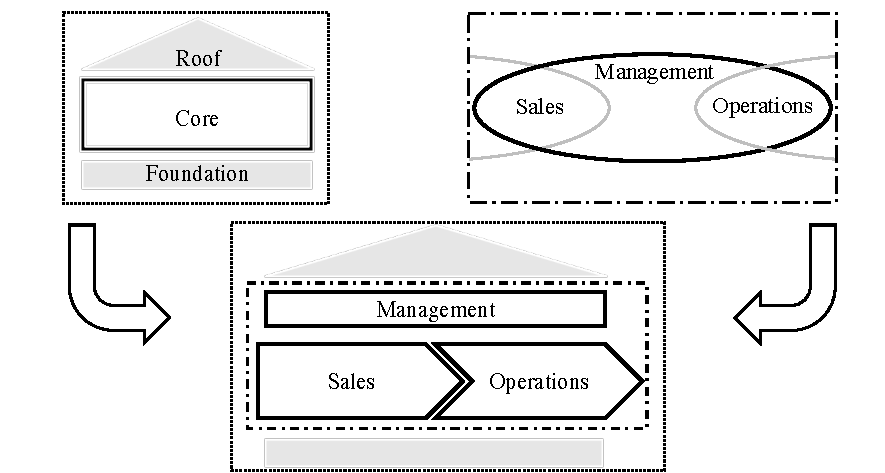
\includegraphics[width=.8\textwidth]{figures/frameworkdesign.pdf}}
	\end{figure} 
	
	
	The value chain can be represented by the exclusive use of chevrons that are linked together or it can have one starting element, which is a pentagon. This element is \textit{closed} to the left side in contrast to the \textit{open} chevrons. Porter uses the \textit{closed} variant, where the increased interface to the left side is emphasized. As the left side of the framework represents the client side, the strong link to the outsourcing partner shall be highlighted \wrt the customer-facing right hand side. Here, the interface to the customer shall be pointed for the following reasons. First, the interaction with a customer is intended to be independent of communication channel, so that the idea of omni-channel is conveyed. Second, the customer-centric idea is communicated with this representation, as all actions towards him (the complete height of the chain) is pinpointed towards one customer. The process structure of three elements consequently locates sales processes on the left and starting part of the value chain and connects the operations processes with it, so that the client and customer side is represented. The value chain is deliberately wider than the house, 
	
	The management processes are located above the value chain and spans the complete width of the house. While it is part of the core, it does not have a \acrshort{VACD} representation, as it has little contact with the the client or customer. However, it influences the complete part of business and is a indispensable part of the \acrshort{BPO} provider business, hence it must be part of the core instead of the roof. Sales processes benefit from the product and portfolio management, while workforce- and agent-related processes are scoped towards service delivery and with it operations. The reason for locating it at the top of the \acrshort{VACD} is that these processes include tactical to strategical aspects, that influence the underlying processes in the framework's core. 
	
	\subsubsection{Framework details}
	
	Locating the identified processes on the framework needs to be done carefully, as their position and shape is important for the viewer's perception. The three areas of the framework's core narrow down positioning alternatives. Their size and shape is equal, to emphasize their main process feature. Customer facing processes vary slightly. Support and Coordination processes have a smaller boxes, font size and slimmer boarders to limit their attention. \Fig \ref{fig:framework} shows the framework.
	
		\begin{figure}[caption={Framework}, label={fig:framework}]
		{	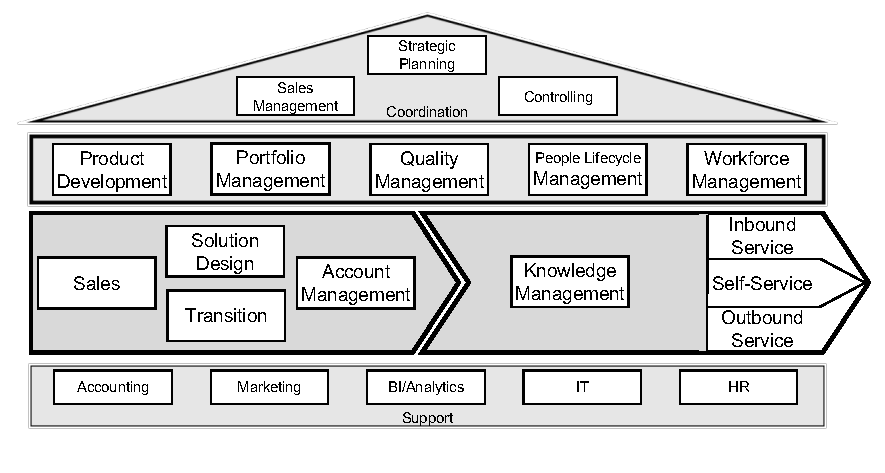
\includegraphics[width=.8\textwidth]{figures/framework.pdf}}
	\end{figure} 
	
	
	 Starting with sales-related processes, the main processes Sales, Solution Design, Implementation and Account Management have to be placed on the framework. As explained in \ref{sec:procstr}, they follow a life cycle, so that Sales leads to Solution Design and Implementation, while existing clients relationships are cared in account management. This leads to a positioning of Sales as the leftmost and account management as the rightmost process within the sales area. Implementation and Solution Design are processes that take between the previous ones.They are both part of the setup of a business and are hence located next to each other. 
	 
	 Operations processes have the peaked customer interface as starting point for locating processes. The split into inbound, outbound and self service as customer facing processes, that are accompanied by knowledge management as an process that takes place without knowledge of the customer. Consequently, knowledge management is located towards the center of the framework and less directed to the customer. The other three processes share their direct customer contact and are therefore in the right part of the chevron. To emphasize their role as the interface to the customer, their representation is adjusted to link to the customer. Furthermore, they are also located on the same height in the flow of the chain to highlight that these are alternatives of contact. By making no distinction of channels on framework level, their equality of treatment is represented. Inbound is written on top, as it is the most important process by volume in among the three, when one sets focus on customer service.
	 
	 The four management processes are located next to each other in their area on top of the \acrshort{VACD}. The product and portfolio process has more connection to the client side, as these service products are sold to the clients. The product development process has a stronger external relation, as new products should meet unsatisfied demands from the market. Portfolio management on the other hand is an intra-organizational process that sets its focus on the provider. The other two processes, namely People  Management and Workforce Management impact the \acrshort{CSR}s. Their positioning can be reasoned through an higher impact of workforce management on the service delivering activities, through schedules, plans and forecasts of customer demand. People Lifecycle Management on the other hand is again oriented towards the provider organization, because the management of human resources for service delivery is of direct interest for the provider, but not to the customer.
	 
	 Support and coordination processes are not further specified in this thesis. Their elements are inspired by general processes of companies, that play a role in \acrshort{BPO}. Processes like accounting or marketing are obvious to fulfill financial regulations and position the provider on the market, respectively. \acrfull{BI} / Analytics captures the process of supporting the business through data-driven insights apart from implemented solutions, as well as to provide decision-support for management on a tactical or strategic level. The latter emphasizes especially  \acrshort{BI} aspect and would also make a positioning in the roof considerable. However, analytics was added to this process as no clear border between the two can be defined in the literature \citep{mertens}. Interpretation of the two notions will vary in an application, as it depends on the understanding in the target organization. IT supports the business through operation of systems (for instance in accounting, HR or for decision-support in management). HR manages people in the provider organization and is different from People Lifecycle Management, as it focuses on \acrshort{CSR}s, not personnel management in general. Sales Management as a coordination process is subject to planning of client businesses and verticals. It is located on the left side of the roof to move it closer to the sales processes. Strategic Planning guides the provider organization as a whole with a long-term perspective. It is located highest in the roof to emphasize its importance for the strategic management of the organization. Controlling completes the coordinating processes by supplying the management with information and overseeing the client businesses. 
	 	 
	 \subsubsection{Addressing  the design goals}
	 
	 	 	\begin{table}[caption={Design Goals}, label={tab:desobj}]
	 	\centering
	 	\begin{tabular}{l p{13.3cm}}
	 		
	 		\textbf{No. }&\textbf{ Design Goal}
	 		\\ \hline
	 		\textbf{1 }                        & The framework has to visualize the business of BPO providers.                                     \\ \hline
	 		\textbf{2}                         & The framework has distinguish business processes from other process types.                                                                                                                   \\ \hline
	 		\textbf{3 }                        & The framework has to cover the CRM-orientation in service provision. \\ \hline
	 		\textbf{4}                         & The framework has to be easily processable by viewers without further explanation.                                                              
	 		
	 	\end{tabular}
	 \end{table}
 
	 
	 With the proposed framework shown in \Fig \ref{fig:framework}, the four design goals are achieved. Its fundamental structure with the \acrshort{VACD} shows encapsulates the BPO business and by exchange of the right chevron, one can apply the model to other domains than \acrshort{CRM}. The relevance of business processes is highlighted through use of the house reference design. The right chevron is suited to represent service delivery in  \acrshort{CRM} through focus on customer contact, while abstracting from explicit processes for offered services (products). These are contained in the product development, solution design and portfolio management process without specifying of measures. Naming these would conflict with the intent of a reference model, as these will be different for companies in the domain. A minimalistic two dimensional representation without additional distracting features such as color or varying fonts supports understanding of the framework. The different shapes are limited and the use of rectangles is preferred. Other elements, like the \acrshort{VACD}, are associated by the viewer and naturally convey the flow of the framework: the outsourcing client's \acrshort{CRM} is given to the provider, who then adds the value to the chain and sends it to the customer. It is noted that application of the reference model results in differences in content, but also in design (to conform to corporate design for instance). However, an empirical evaluation of this framework design was not conducted so statements about viewer's opinions are derived from design choices of the author. 
	 
	 The following dives into the process models below the framework. The icebricks language is used to meet solution objective 4 and hence the underlying structure below the main processes on the framework is composed of detail processes, which in turn have process building block underneath. 
	 
	%%%%%%%%%%
	\section{Management Processes}
	%%%%%%%%%%
	%%%%%%%%%%
	\subsection{Product Development}
	
	\subsection{Portfolio Management}
	
	\subsection{People Lifecycle Management}
	gross bord 98
	
	\subsection{Workforce Management}
	
	%%%%%%%%%%
	%%%%%%%%%%
	\section{Client Processes}
	%%%%%%%%%%
	%%%%%%%%%%
	\subsection{Sales}
	gross 154 rfi rfp
	%birgit1, docs
	\subsection{Solution Design}
	%wollenberg, hybride leistungsbündel .. vielleicht oben noch rein 
	\subsection{Implementation}
	gross 160
	%birgit2, docs, software einführung
	\subsection{Account Management}
	%wiebel, docs, lit
	gross 160
	%%%%%%%%%%
	%%%%%%%%%%
	\section{Customer Processes}
	
	This section describes the Inbound, Outbound, Self-Service and Knowledge Management process. They describe the processing of transactions in the outsourcing contract and are driven by the target domain (\acrshort{CRM}). 
	
	There are several constructs by means of data, that encompass all means of contact to the outsourcing provider. First, every contact involves a customer that is asking for something or more generally put has a lack of information that should be addressed. This lack is possibly related to a product\footnote{Product here encompasses everything that is provided by the client to the market, \ie, services as well.} of the client (be it an actual purchase or solely the consideration), which is denoted as a transaction. Transactions also cover touch points like past customer service contacts or other events between the customer and the company. Together, these product-related and touch point-related transactions are determinants for forming a complete view of the customer. Transactions have a hierarchy, so that one transaction may have to a superior transaction. 
	
	Here, it is assumed that every transaction is related to a customer. Even if it is a new customer, the act of contacting implies a previous touch point with the company. It is noted that this transaction might be not known to the company. A customer can have multiple transactions. The contact happens as an inbound (customer contacts company), outbound (company contacts customer) or self-service (customer reaches company with no involvement of a \acrshort{CSR} ). 
	
	Knowledge bases accessible by the outsourcing provider contain knowledge that is able to address the customer's issue that is reason for contact. As these issues are classifiable, structuring them leads to business cases that describe the solution to a known customer problem. Examples can the cancellation of a booking, the termination of a contract or change of address. This listing reveals that business cases are very dependent on the business of the client and hence are not a valid criterion for structuring customer contacts in a reference model. Not every customer contact needs to relate to a case. The \acrshort{ERM} in \Fig \ref{fig:contacterm} shows the described circumstances around the contact. It also reasons the structuring of the knowledge management process. 
	
	\begin{figure}[caption={Framework}, label={fig:contacterm}]
		{	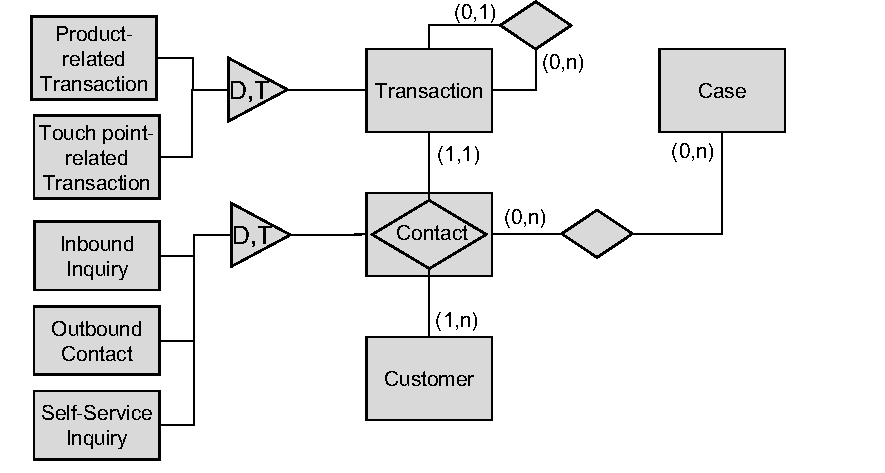
\includegraphics[width=.8\textwidth]{figures/contacterm.pdf}}
	\end{figure} 

	
	This analysis is necessary due to the complex and highly variable processes in Customer Service. Process Identification for Customer Service in the field of the After Sales Service as a Basis for “Lean After Sales Service”
	im hippner buch it automation chapter für self service!
	%%%%%%%%%%
	Self Service: Servitization paper 1988!
	
	hippner:692 muss nicht nur inbound sein, outbound geht auch
	
	\subsection{Inbound}
	The associated object to this process in the \textit{inquiry}\footnote{inquiry is American English; enquiry is British English.}. It is preferred over \textit{request} as it emphasizes an investigation in an issue over the politeness during asking. It is defined as an act of asking for information \citep{oxfordenquiry, oxfordrequest}. In this case, it is the customer who is lacking information in some regard and contacts the company. A \acrshort{CSR} of the outsourcing provider attends to the matter. 
	
	Reflections on the structure of the process become especially important in case of an omni-channel environment. There are multiple contact channels, asynchronous and synchronous communication and generic reasons that lead to the inquiry. Rationale behind omni-channel process modeling must be to keep the structure channel independent as long as possible to enable alignment. To capture the peculiarities of the channels, the concept of variants is used on the lowest level to distinguish between mail, voice, direct messenger and social channels. Reasons for this split is that other discussed channels (Video, Website, App) can be included in others by means of a process view (video to voice) or are not a contact channel by means of inbound customer service. The website and app are gateways to other channels (direct messenger) or to self-service, but do not offer direct engagement with a \acrshort{CSR}. 
	
	The detail processes are structured so that their steps apply to all channels. This structuring was found to be applicable among the participants in the process modeling workshop and is shown in \Fig \ref{fig:inbproc}. First, the detail processes are described without going into details of their channel-variants. 
	
\begin{figure}[caption={Inbound process}, label={fig:inbproc}]
	\begin{center}
		\begin{tikzpicture}
	[node distance=.5cm, start chain=going below,]
	\node[punktchain, join=by {-}] (eins)      {Route inquiry};
	\node[punktchain, join=by {-}] (zwei) {Preprocess inquiry};
	\node[punktchain, join=by {-}, ] (drei) {Classify inquiry};
	\node[punktchain, join=by {-}, ] (vier) {Process inquiry};
	\node[punktchain, join=by {-}, ] (fuenf) {Review inquiry};
	\end{tikzpicture}
\end{center}
\end{figure}

First, an inbound inquiry reaches is initiated by a customer and the connection with the receiving end is established. Before an interaction starts, the inquiry needs to be guided to a \acrshort{CSR}, which is known as routing in telecommunications. During this \textit{routing} process, information from the caller is processed, so that part of his needs can be inferred before the employee starts the conversation and time (and money) is consumed. On the other hand, time that the customer spends in the system before the conversation is not consuming scarce resources from the provider, so the extraction of information usable to address his problem is desirable. At the end of routing, a \acrshort{CSR} is found that starts the conversation with the customer. In the \textit{preprocessing} step, the \acrshort{CSR} takes on the inquiry and consumes the information that is available from the routing, as well as transmitted by the customer. After this familiarization the \acrshort{CSR} can \textit{classify} the \textit{inquiry}, so that he knows how to map the individual inquiry of the customer to a case (if existent). The\textit{ process inquiry } detail process engages the inquiry and ideally solves the problem. The last step involves a \textit{review}, if applicable to the channel and closes the conversation. This step can be described as post-processing, because data related to the communication is entered and stored in the knowledge base. As every detail process in \Fig \ref{fig:inbproc} has four variants, 
	


\begin{figure}[caption={Exemplary use of subfigures}, label={fig:subfig}]
	
	\begin{subfigure}[b]{.45\textwidth}
		\centering
			\begin{tikzpicture}
		[node distance=.5cm,
		start chain=going below,]
		
		\node[punktchain, join=by {-}] (eins)      {Route inquiry};
		\node[punktchain, join=by {-}] (zwei) {Preprocess inquiry};
		\node[punktchain, join=by {-}, ] (drei) {Classify inquiry};
		\node[punktchain, join=by {-}, ] (vier) {Process inquiry};
		\node[punktchain, join=by {-}, ] (fuenf) {Review inquiry};
		
		\end{tikzpicture}
	
		\caption{eins}\label{fig:subfig1}
	\end{subfigure}
	\begin{subfigure}[b]{.45\textwidth}
		\centering	
		\begin{tikzpicture}
	[node distance=.5cm,
	start chain=going below,]
	
	\node[punktchain, join=by {-}] (eins)      {Route inquiry};
	\node[punktchain, join=by {-}] (zwei) {Preprocess inquiry};
	\node[punktchain, join=by {-}, ] (drei) {Classify inquiry};
	\node[punktchain, join=by {-}, ] (vier) {Process inquiry};
	\node[punktchain, join=by {-}, ] (fuenf) {Review inquiry};
	
	\end{tikzpicture}
		\caption{zwei}\label{fig:subfig2}
	\end{subfigure}
\begin{subfigure}[b]{.45\textwidth}
	\centering	
	\begin{tikzpicture}
	[node distance=.5cm,
	start chain=going below,]
	
	\node[punktchain, join=by {-}] (eins)      {Route inquiry};
	\node[punktchain, join=by {-}] (zwei) {Preprocess inquiry};
	\node[punktchain, join=by {-}, ] (drei) {Classify inquiry};
	\node[punktchain, join=by {-}, ] (vier) {Process inquiry};
	\node[punktchain, join=by {-}, ] (fuenf) {Review inquiry};
	
	\end{tikzpicture}
	\caption{drei}\label{fig:subfig3}
\end{subfigure}
\begin{subfigure}[b]{.45\textwidth}
	\centering	
	\begin{tikzpicture}
	[node distance=.5cm,
	start chain=going below,]
	
	\node[punktchain, join=by {-}] (eins)      {Route inquiry};
	\node[punktchain, join=by {-}] (zwei) {Preprocess inquiry};
	\node[punktchain, join=by {-}, ] (drei) {Classify inquiry};
	\node[punktchain, join=by {-}, ] (vier) {Process inquiry};
	\node[punktchain, join=by {-}, ] (fuenf) {Review inquiry};
	
	\end{tikzpicture}
	\caption{vier}\label{fig:subfig4}
\end{subfigure}
\end{figure}


	
	 
	\subsection{Self Service}
	\subsection{Outbound}
	%%%%%%%%%%
	%%%%%%%%%%
	%%%%%%%%%%
